\hypertarget{a00012}{
\section{Dokumentacja klasy ASS8.Klient.klientUsun}
\label{df/d86/a00012}\index{ASS8::Klient::klientUsun@{ASS8::Klient::klientUsun}}
}
Klasa zawiera dane do serializacji zapytania o usunięcie pliku.  


Dziedziczy \hyperlink{a00007}{ASS8::Klient::klientBase}.

Diagram współpracy dla ASS8.Klient.klientUsun:\nopagebreak
\begin{figure}[H]
\begin{center}
\leavevmode
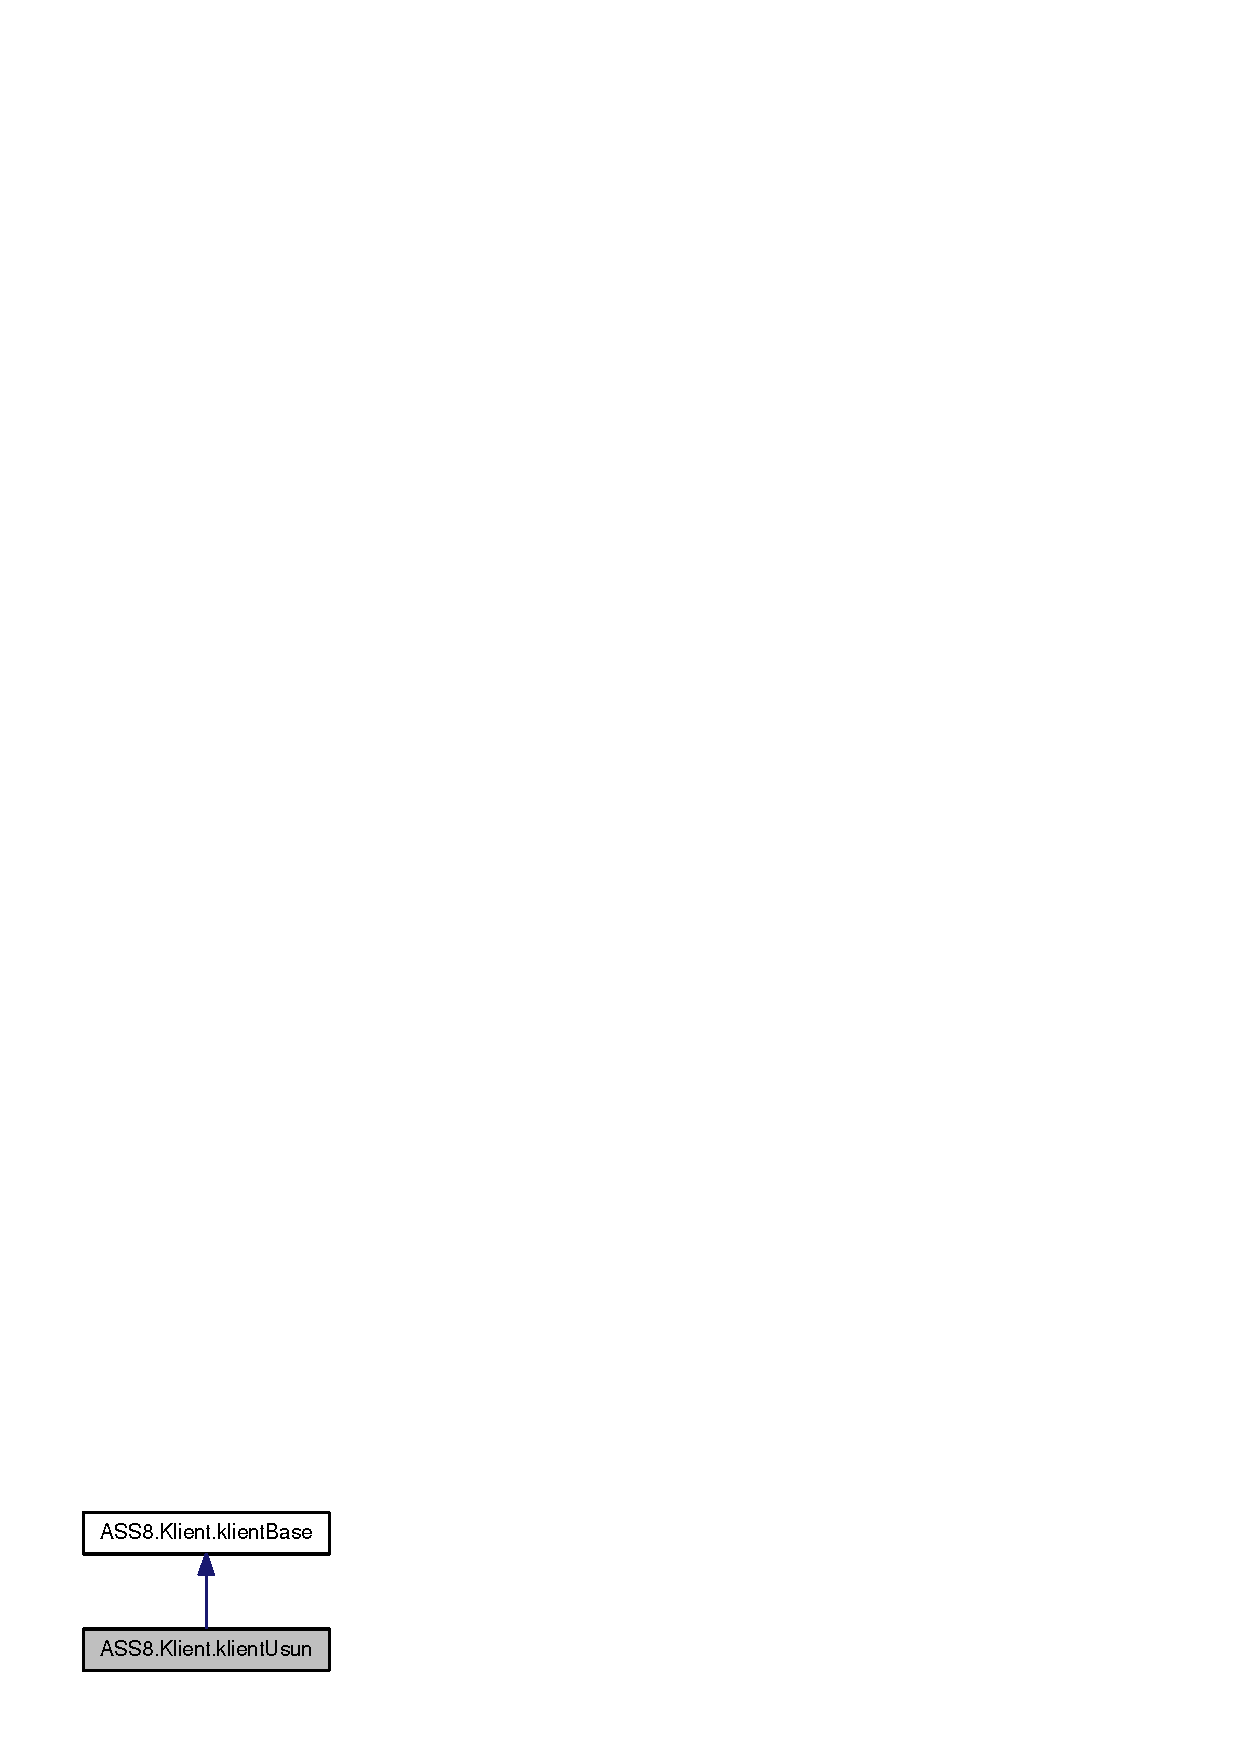
\includegraphics[width=162pt]{d1/d72/a00204}
\end{center}
\end{figure}
\subsection*{Metody publiczne}
\begin{CompactItemize}
\item 
\hyperlink{a00012_b199284c747db6951ae55f6276bb80f3}{klientUsun} ()
\item 
\hyperlink{a00012_deeafd41f76b7ec30ef021354ea80cb8}{klientUsun} (int id, int oper, List$<$ \hyperlink{a00018}{plikInfo} $>$ pi)
\end{CompactItemize}
\subsection*{Właściwości}
\begin{CompactItemize}
\item 
List$<$ \hyperlink{a00018}{plikInfo} $>$ \hyperlink{a00012_65f1c0b67462c058fc083489a442d824}{plik}\hspace{0.3cm}{\tt  \mbox{[}get, set\mbox{]}}
\end{CompactItemize}
\subsection*{Atrybuty prywatne}
\begin{CompactItemize}
\item 
List$<$ \hyperlink{a00018}{plikInfo} $>$ \hyperlink{a00012_c82991917146a9f234484a6b3e5ad685}{pPlik}
\end{CompactItemize}


\subsection{Opis szczegółowy}
Klasa zawiera dane do serializacji zapytania o usunięcie pliku. 



Definicja w linii 334 pliku XmlRequestsClass.cs.

\subsection{Dokumentacja konstruktora i destruktora}
\hypertarget{a00012_b199284c747db6951ae55f6276bb80f3}{
\index{ASS8::Klient::klientUsun@{ASS8::Klient::klientUsun}!klientUsun@{klientUsun}}
\index{klientUsun@{klientUsun}!ASS8::Klient::klientUsun@{ASS8::Klient::klientUsun}}
\subsubsection[{klientUsun}]{\setlength{\rightskip}{0pt plus 5cm}ASS8.Klient.klientUsun.klientUsun ()}}
\label{df/d86/a00012_b199284c747db6951ae55f6276bb80f3}




Definicja w linii 337 pliku XmlRequestsClass.cs.\hypertarget{a00012_deeafd41f76b7ec30ef021354ea80cb8}{
\index{ASS8::Klient::klientUsun@{ASS8::Klient::klientUsun}!klientUsun@{klientUsun}}
\index{klientUsun@{klientUsun}!ASS8::Klient::klientUsun@{ASS8::Klient::klientUsun}}
\subsubsection[{klientUsun}]{\setlength{\rightskip}{0pt plus 5cm}ASS8.Klient.klientUsun.klientUsun (int {\em id}, \/  int {\em oper}, \/  List$<$ {\bf plikInfo} $>$ {\em pi})}}
\label{df/d86/a00012_deeafd41f76b7ec30ef021354ea80cb8}




Definicja w linii 338 pliku XmlRequestsClass.cs.

\subsection{Dokumentacja atrybutów składowych}
\hypertarget{a00012_c82991917146a9f234484a6b3e5ad685}{
\index{ASS8::Klient::klientUsun@{ASS8::Klient::klientUsun}!pPlik@{pPlik}}
\index{pPlik@{pPlik}!ASS8::Klient::klientUsun@{ASS8::Klient::klientUsun}}
\subsubsection[{pPlik}]{\setlength{\rightskip}{0pt plus 5cm}List$<${\bf plikInfo}$>$ {\bf ASS8.Klient.klientUsun.pPlik}\hspace{0.3cm}{\tt  \mbox{[}private\mbox{]}}}}
\label{df/d86/a00012_c82991917146a9f234484a6b3e5ad685}




Definicja w linii 336 pliku XmlRequestsClass.cs.

\subsection{Dokumentacja właściwości}
\hypertarget{a00012_65f1c0b67462c058fc083489a442d824}{
\index{ASS8::Klient::klientUsun@{ASS8::Klient::klientUsun}!plik@{plik}}
\index{plik@{plik}!ASS8::Klient::klientUsun@{ASS8::Klient::klientUsun}}
\subsubsection[{plik}]{\setlength{\rightskip}{0pt plus 5cm}List$<${\bf plikInfo}$>$ ASS8.Klient.klientUsun.plik\hspace{0.3cm}{\tt  \mbox{[}get, set\mbox{]}}}}
\label{df/d86/a00012_65f1c0b67462c058fc083489a442d824}




Definicja w linii 345 pliku XmlRequestsClass.cs.

Dokumentacja dla tej klasy została wygenerowana z pliku:\begin{CompactItemize}
\item 
\hyperlink{a00055}{XmlRequestsClass.cs}\end{CompactItemize}
